\chapter{Intelligence Artificielle - Algorithme}

	\section{Éléments techniques}
	
\paragraph{Algorithme (4.1.2.) :}
Un algorithme est une suite finie et non ambiguë d’opérations 
ou d'instructions permettant de résoudre une classe de problèmes.

https://fr.wikipedia.org/wiki/Algorithme

\paragraph{Arbre (4.1.2.) :}
Un arbre en informatique est consititué d'arêtes (appelé branche),
d'états non finis (appelé noeud) et finis (appelé feuille). Chaques
branches mênent à un état à l'aide d'une action à partir d'un état
précédent (père). On appelle feuille un état qui ne possède pas d'état 
suivant (fils). La racine de l'arbre est appelé l'état initial.

\paragraph{Algorithme MinMax (4.1.2.) :}
L'algorithme minimax (aussi appelé algorithme MinMax) est un 
algorithme qui s'applique à la théorie des jeux1 pour les jeux à 
deux joueurs à somme nulle (et à information complète) consistant à
minimiser la perte maximum (c'est-à-dire dans le pire des cas).

https://fr.wikipedia.org/wiki/Algorithme\_minimax

\paragraph{Profondeur de recherche (4.1.4.):}
La profondeur de recherche dans les algorithmes s'appliquant à la
théorie des jeux, est la limite du niveau qui peut être parcouru
depuis l'état initial aux noeuds de l'arbre.

			
	\section{Nécessités}
	\paragraph{Comment gagner au jeu de Tron?}
	Pour jouer une partie, le programme doit savoir prendre une décision    sur la direction que doit emprunter un joueur. La façon la plus pratique est    de simuler tous les déplacements possibles à partir d'une position donnée,     puis répéter ce processus sur plusieurs tours de jeu. Ce qui permet d'arriver    à une partie finie ou un état du plateau qui pourrait exister. 
	
	
	\section{Problème}
	
	\paragraph{Comment générer un arbre* d'états, dans une partie à plusieurs joueurs ?}
	
	Il existe plusieurs styles d'algorithmes* permettant de résoudre des    problèmes différents. Pour notre sujet, nous devons utiliser des algorithmes     s'appliquant à la théorie des jeux. Le principe de l'algorithme MinMax*    permettrait de trouver un déplacement idéal sur le plateau du jeu Tron, cet    algorithme fonctionne pour les jeux à deux joueurs à sommes nulles, nous ne    pouvons pas l'utiliser. En essayant de nous inspirer de son principe, nous    pourrons générer un parcours dans l'arbre étant évalué par une heuristique*.  
	
	
	\section{Approches possibles}
	\paragraph{Algorithme Paranoide}
	L'algorithme paranoïde fonctionne sur le principe de celui de MinMax,     une des différences qui existe entre ces deux algorithmes est qu'il     s'applique sur la théorie des jeux pour plusieurs joueurs. Cet     algorithme part du principe que tous les joueurs du terrain sont     contre lui, tous les joueurs adverses choisiront donc la perte      maximum du joueur et lui minimisera sa perte. 
	
	L'algorithme paranoïde à hauteur de sa profondeur de recherche* ne     pourra pas se tromper. En revanche, il n'est pas garanti que le meilleur coup actuel ne soit pas le pire coup au tour suivant.  
	
	\paragraph{Algorithme de Monte-Carlo}
	L'algorithme de Monte-Carlo fonctionne sur le principe de l'aléatoire.
	Cet algorithme n'as pas besoin d'une fonction d'heuristique explicite pour fonctionner, pour déterminer la valeur d'une situation, il lui suffit de determiner des coups au hasard, puis de jouer les états de parties résultantes de ces coups pour faire une moyenne des défaites et victoires. Les coups ayant une succession de coups le plus victorieux sont alors considérés comme les coups les plus intéressants potentiellement.
	
	L'algorithme Monte-Carlo est très rapide, et donné un temps infini de calcul, converge vers le résultat d'un min max, mais sa version de base converge lentement et son approche algorithmique n'est pas triviale pour un niveau de licence.
	
	\section{Approche utilisée}
	\paragraph{Algorithme Negamax avec élagages}
	Afin d'obtenir un maximum de résultat dans la phase de l'    analyse, nous devons avoir un algorithme rapide. L'algorithme Monte-Carlo    pourrait être une solution sur la rapidité, avec l'expérience du groupe,    nous avons choisi l'algorithme paranoïde sous forme négamax qui semble être le plus facile à    réaliser dans le temps de ce projet. Pour optimiser le temps de calcul, nous    avons rajouté quelques élagages pour l'accélérer.
	
	\paragraph{Élagage Alpha-Bêta}
	L'élagage alpha bêta est une technique permettant de couper les    branches de l'arbre qui représente des sous-arbres possédant des valeurs    qui ne contribuent pas au calcul minmax de notre algorithme.
	
	\section{Remarques sur les résultats obtenus}
	
	\paragraph{Aucun déplacement trouvé}
	Lorsque l'algorithme paranoïde perçoit la fin de son équipe dans    toutes ces branches, vu que l'heuristique est une évaluation par rapport au     terrain (en effet vu que l'équipe est morte l'heuristique renverra 0). Il    sera incapable de faire la différence entre ces états menant vers sa fin,     l'algorithme renverra la première action, donné dans la liste d'actions    possible. Pour éviter ce genre d'événement, nous avons ajouté à    l'algorithme une détection d'action permettant de déterminer si l'algorithme    n'a pas trouvé de solutions. L'algorithme choisira un coup aléatoire parmi les actions possibles, qui ne tuera pas le joueur.
	
	\paragraph{Phénomène d'horizon}
	Nous avons observé un phénomène lors de nos tests de l'algorithme
	paranoïde. Le joueur seul pense que la partie est finie et passe dans le
	mode survie de l'algorithme expliqué ci-dessus*, alors qu'il pouvait s'en sortir.
	
	En effet nous avons vu que l'une des faiblesses de cet algorithme 
	est que nous ne sommes pas garantis de la fiabilité du coup choisie au tour
	suivant. Vu que le joueur seul a une vision plus profonde de la partie que
	ses adversaires, il perçoit l'opportunité de ses adversaires de le tuer.
	Mais si cette opportunité est vue dans une profondeur plus grande que celle
	de l'adversaire alors elle n'est pas garantie d'arrivée, car l'adversaire
	jouera le meilleur coup à hauteur de sa profondeur. Ce phénomène fournit une
	preuve de la limite de puissance de l'algorithme paranoïde. 
	
	Nous avons vu l'impact le plus gênant de ce phénomène, mais nous
	pouvons aussi remettre en cause avec le même principe, tout les calculs pris
	en compte lorsque la profondeur d'un joueur dépasse celle de son adversaire.
	En effet lorsque les calculs sont faits dans des hauteurs de profondeur
	accessible par tous les joueurs, les joueurs percevront les états futurs.
	En revanche dès que la profondeur dépasse la profondeur de l'adversaire, le
	joueur obtient une prévision des meilleurs états futurs de son adversaire.
	Il jouera le meilleur coup possible en fonction de ces états, mais ce coup
	n'étant pas calculé dans les autres états futurs possibles, ce coup ne sera
	plus le meilleur coup possible (remarque: dans la majorité des cas il reste
	un coup assez viable).
	
	\section{Pistes d'améliorations}
	\paragraph{Concernant l'optimisation de temps d'éxecution}
	Lorsque l'algorithme détecte à hauteur de sa profondeur que la 
	partie est finis, il arrête de jouer le meilleur coup possible et joue des
	coups aléatoires. Après chaque coup l'algorithme est rappelé, ce qui
	ralentit grandement l'analyse de résultat. Nous pourrions retirer le mode
	survie de l'algorithme, et déclarer un vainqueur par abandon. Mais nous
	avons vu que l'algorithme peut se tromper lorsque sa profondeur est plus
	grande que l'adversaire.
	
	Nous avons observé plusieurs fois des situations où l'algorithme
	prévoit qu'il va perdre. Ces prévisions ont 75\% d'être vrai.
	
	Conclusion, si nous utilisons cette amélioration nous perdrons en
	précision de résultat, mais nous gagnerons plus en temps d'exécution de
	l'analyse.
	
	\paragraph{Concernant le phénomène d'horizon}
	Il existe l'algorithme Expectimax qui va jouer des coups aléatoires et
	faire une moyenne. Nous pourrions garder notre algorithme paranoïde, puis
	lorsque la profondeur dépasse celle de l'adversaire alors les coups des
	adversaires seront joués aléatoirement et une moyenne sera faite à partir de
	ce niveau. 


\chapter{Intelligence Artificielle - Heuristique}

\section{Éléments techniques}

\paragraph{Heuristique (4.1.3.) :}
Une heuristique permet de faire une évaluation d'un état, afin de
différencier un état d'un autre. Ces différences permettent aux
algorithmes de faire un choix entre plusieurs actions.

\section{Nécessités}

\paragraph{Évaluation du plateau}
Lors d'une partie de jeu Tron, le joueur qui possède la plus grosse
zone de contrôle sur le plateau gagnera. En partant sur cette stratégie,
l'heuristique devra calculer la zone de contrôle des joueurs.

\section{Problème}

\paragraph{Comment pourrions-nous faire une heuristique rapide, mais aussi donnant
des résultats fiables ?}
L'heuristique devra évaluer la valeur d'une situation. Devant
parcourir tout le plateau, pour évaluer un état, il faudra beaucoup de 
calculs pour obtenir une valeur précise. Il nous faudra être suffisamment
rapides sur cette partie afin de générer assez de tests pour l'analyse des
configurations de la partie.

\section{Approche possible}

\paragraph{Parcours de recherche BFS pour un joueur}
Ce parcours va calculer la distance de chaque case depuis la
position du joueur, cette opération est répétée pour tous les joueurs.
L'attribution de la case est donnée à l'équipe possédant la plus petite
distance sur cette case. La complexité de l'heuristique est de 
n * m * c.

\paragraph{Parcours de recherche BFS joueur par joueur}
Dans cette approche, le parcours BFS va s'étendre à partir de tous 
les joueurs. La complexité de l'heuristique est de n*m.

\paragraph{Évaluation de la zone de contrôle en nombre de cases possédé}
lorsque nous évaluons un plateau en nombre de cases, minimiser
signifie réduire la taille de la zone du terrain contrôlé par le joueur.
Sauf que réduire la zone adversaire ne signifie pas forcément augmenter la
sienne. L'algorithme paranoïde minimise la zone du joueur lors de la 
simulation du coup de son adversaire, alors que l'adversaire à son tour
essayera de maximiser sa zone. Nous nous retrouvons dans un état qui n'a
pas été prévu par l'algorithme et donc fausse toute la perception des états
futurs calculée par l'algorithme.

\begin{figure}[H]
	\centering
	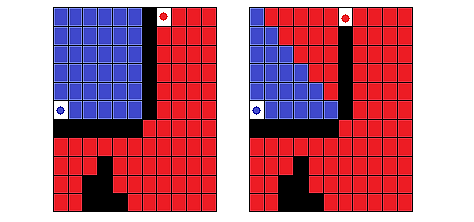
\includegraphics[width=0.8\textwidth, keepaspectratio, height=0.2\textheight]{./pics/nbr_case.png}	
	\caption{bleu = 20 cases/ 20\% ; rouge = 82 cases/ 80\%}
\end{figure}

\begin{figure}[H]
	\centering
	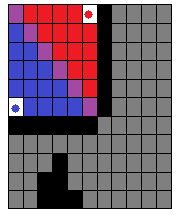
\includegraphics[width=0.8\textwidth, keepaspectratio, height=0.2\textheight]{./pics/nbr_case_mini.png}	
	\caption{bleu = 14 cases/ 50\% ; rouge = 14 cases/ 50\%}
\end{figure}

\begin{figure}[H]
	\centering
	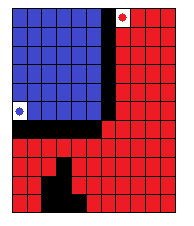
\includegraphics[width=0.8\textwidth, keepaspectratio, height=0.2\textheight]{./pics/nbr_case_maxi.png}	
	\caption{bleu = 35 cases/ 35\% ; rouge = 66 cases/ 65\%}
\end{figure}


\paragraph{Évaluation de la zone de contrôle en pourcentage du terrain jouable
possédé}
L'évaluation d'une zone contrôle convertit en pourcentage de
contrôle du terrain jouable, permet d'obtenir une heuristique à sommes nulle
. En effet lorsqu'un joueur maximise son pourcentage de contrôle du terrain,
il diminuera celui de son adversaire et vice-versa.

\section{Approche utilisée}

\paragraph{ Parcours de recherche et Optimisation}
Il est évident que nous allons utiliser l'approche avec la meilleure
complexité. Cette méthode est rapide pour sa fiabilité, mais lors de
l'exécution de l'analyse de donnée, cette partie est la plus coûteuse de 
notre simulation.

Notre principal objectif est d'obtenir suffisamment de résultats,
afin de déduire qu’elles seront les paramètres idéaux pour résoudre la
problématique. Avec notre calcul de la zone de contrôle, les estimations de
calcul s'élèvent à plus de 48H.

Pour améliorer le temps de calcul de la zone de contrôle, on
suppose que le joueur seul possède moins de terrain que la coalition et
qu'une zone qu'il ne contrôle pas est une zone appartenant à la coalition.

Avec ces suppositions on remarque que les cases isolées (voir case 
grise de l'image tag 2) n'appartiennent à aucune équipe. Avec cette
supposition on constate qu'une case que ne possède pas le joueur seul n'est
pas forcément une case appartenant à son adversaire. Utiliser ce principe
nous ferait gagner en temps de calcul, mais nous perdrons en fiabilité.

Pour générer cette amélioration, l'heuristique calculera la zone de 
contrôle de chaque équipe, le parcours BFS sera interrompu lorsque le
joueur seul ne peut plus obtenir de case pour sa zone de contrôle. En effet
avec cette solution la zone de contrôle des joueurs de la coalition risque
de ne plus être calculée en entier. Pour obtenir la zone de contrôle de la
coalition, une approximation de celle-ci va s'ajouter aux calculs de
l'heuristique. 

À partir de la zone de contrôle du joueur seul et la taille du
terrain jouable (le nombre de cases libre), nous pouvons en déduire une
approximation de la zone contrôlée par la coalition.
(ex. : 	
zone contrôle seule = (cases possédées / terrain jouables) * 100
zones contrôle coalition = 100 - zone contrôle seule
)

\begin{info}
	Dans cette approche, nous ne sommes plus obligés de calculer toutes
	les cases du terrain jouable. En effet toutes les cases d'une zone ne sont
	plus calculées lorsqu'une zone est plus grande que la zone du joueur seul.
\end{info}

\begin{figure}[H]
	\centering
	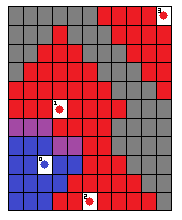
\includegraphics[width=0.8\textwidth, keepaspectratio, height=0.25\textheight]{./pics/heuristique_interruption.png}	
	\caption{Calcul de la zone de contrôle du joueur 3}
\end{figure}

Avec cette méthode, nous gagnons en temps d'exécution et nous
perdons en fiabilité (à cause des cases isolée et constatée). Le moyen
d'augmenter la fiabilité serait d'améliorer l'approximation, mais sans
calculer la zone de contrôle de la coalition. L'estimation de calcul
s'élève désormais à 24H, ce qui est toujours élevé.

On remarque qu'un joueur trop éloigné n'aura pas d'impact sur le 
calcul de la zone de contrôle du joueur seul. On considéra un joueur trop
éloigné lorsqu'il est éloigné sur une distance de deux fois supérieure à 
celle de la profondeur du joueur seul. Avec une distance deux fois supérieure
à celle de la profondeur du joueur seul, même si les deux joueurs se
rapprochent tout le long des tours, la distance est telle, qu'à la fin de la
recherche ils ne pourraient toujours pas interagir l'un avec l'autre.

Vu que l'heuristique va calculer une zone qui n'a pas d'impact sur la
zone de contrôle du joueur seul, nous pouvons supprimer tous les joueurs qui
sont trop éloignés du joueur seul. En effet au début du calcul de
l'heuristique, nous initialisons la position de départ de chaque joueur.
Grâce à la distance de Manhattan entre les joueurs, nous pouvons déterminer
les joueurs assez proches et les prendre en considération lors du calcul des
zones.

\begin{info}
	Perde en fiabilité n'est pas forcement un point négatif lors de
	la phase d'analyse. En effet grâce à l'optimisation des temps de calcul nous
	pouvons générer beaucoup plus de résultats. Parmi ses résultats les petites
	erreurs de fiabilité seront noyées dans la masse d'information, car nos
	erreurs de fiabilité ne sont pas une généralité, mais des cas très
	particuliers de partie.
\end{info}


\section{Remarques sur les résultats obtenus}

\paragraph{Maximiser, minimiser un nombre de cases}

Avec une heuristique basée sur les nombres de cases contrôlées par une
équipe, nous avons constaté que le joueur seul essayait d'augmenter sa zone
alors que les joueurs de la coalition essayaient de réduire la taille du 
joueur seul, dans l'algorithme paranoïde la stratégie des dans camps doit
être identique, ce qui n'est pas le cas avec une telle heuristique.

\section{Observation sur les résultats des coups impliqués par l'heuristique}
\subsection{Déplacement serpent}
Lorsqu’un joueur ne peut plus agir sur la zone de l'adversaire à    hauteur de sa profondeur, l'algorithme se déplace sur toutes les cases    qu'il peut parcourir.



\begin{figure}[H]
	\centering
	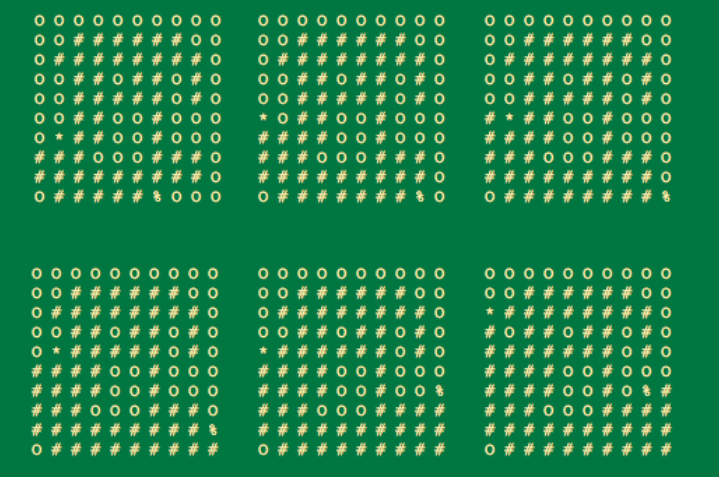
\includegraphics[width=0.8\textwidth, keepaspectratio, height=0.5\textheight]{./pics/serpent.png}	
	\caption{Observation d'un déplacement en serpent}
\end{figure}

\subsection{Abandon lors de la mort}

Dès que l'algorithme détecte sa mort à hauteur de sa profondeur    (donc cette information peut être fausse), tous les états futurs ne    peuvent être différenciés, nous avons rajouté un mode survie le permettant    de continuer à survivre en espérant que la situation puisse s'améliorer.



\begin{figure}[H]
	\centering
	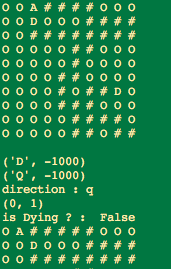
\includegraphics[width=0.8\textwidth, keepaspectratio, height=0.3\textheight]{./pics/anti_suicide.png}	
	\caption{Changement de déplacement avec le filtre de situation}
\end{figure}



\subsection{Stratégie}
Dans la stratégie de posséder une plus grande zone de    contrôle que son adversaire, se rapprocher de son adversaire est une bonne    manière de diminuer la zone de contrôle de son adversaire. Cette situation    peut se produire lorsqu'un joueur peut diminuer la zone de son adversaire    tout en augmentant la sienne. Dans le même cas de situation, un joueur peut    enfermer un adversaire dans une partie du terrain.


\begin{figure}[H]
	\centering
	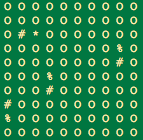
\includegraphics[width=0.8\textwidth, keepaspectratio, height=0.2\textheight]{./pics/rapprochement.png}	
	\caption{Observation de rapprochement des joueurs}
\end{figure}


\begin{figure}[H]
	\centering
	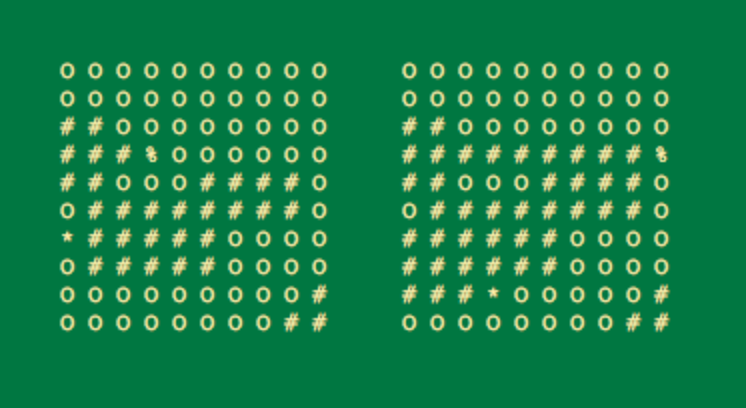
\includegraphics[width=0.8\textwidth, keepaspectratio, height=0.4\textheight]{./pics/enfermement.png}	
	\caption{Observation d'un enfermement}
\end{figure}

Ces comportements sont nés de l'heuristique, mis à part le mode survie.
Changer l'heuristique affectera ces comportements.


\subsection{Sacrifice}
Le mode survie doit pouvoir faire la différence entre un suicide    pour l'équipe et un abandon. Un joueur de la coalition peut s'apercevoir    que sa présence sur le plateau n'est pas bénéfique à l'équipe, il devra    se retirer du plateau en se tuant.


\begin{figure}[H]
	\centering
	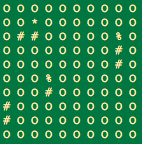
\includegraphics[width=0.8\textwidth, keepaspectratio, height=0.2\textheight]{./pics/sacrifice.png}	
	\caption{Sacrifice pour l'équipe}
\end{figure}


\section{Pistes d'amélioration}
Une autre solution serait de modifier l'heuristique en ajoutant à son 
évaluation d'un plateau, le nombre de joueurs présents sur le plateau, le
nombre de tour, la taille de la zone de contrôle du terrain adverse. Ce qui
permettrait de rajouter plus d'évaluation sur un état lorsqu'un joueur
possède une zone de contrôle faible.

